\chapter{Third week}
\section{EDA}
After finishing last week's statistics assignments, it is time to analyse the entire dataset we'll be working with.
The data we've hitherto been working with consisted of three files:
\begin{itemize}
    \item Expression data where columns are samples and rows are genes.
    \item Gene annotations to match genes to their chromosome.
    \item Cancer type annotations to match samples to their cancer type.
\end{itemize}
Now that the phase of demonstration is over, we've received the following data:
\begin{itemize}
    \item A mixing matrix where columns are transcriptional components and rows are genes with an approximate shape of 10k x 10k.
    \item A larger set of cancer type annotations.
\end{itemize}

This mixing matrix is the data we'll use for machine learning later in this project to generate annotations eventually.
However, before we can do that, we will perform an exploratory data analysis

\subsection{Distributions of basic statistics}
This new dataset came with a new set of assignments, the first of which was to plot the distributions of some statistical values.
The values in question are:
\begin{itemize}
    \item Minimum
    \item Maximum
    \item Mean
    \item Median
    \item Standard deviation
    \item 1$^{st}$ quartile
    \item 3$^{rd}$ quartile
\end{itemize}
These distributions were to be visualised using histograms, where each histogram would display the distribution of a statistic.
Below, all seven histograms can be found.

\begin{figure}[H]
    \centering
    \begin{subfigure}[t]{.3\textwidth}
        \centering
        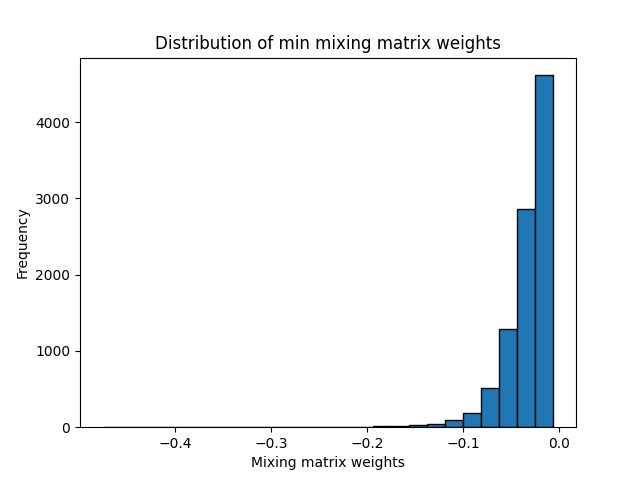
\includegraphics[scale=0.3]{mm_min}
        \caption{Distribution of minimal weights for every TC}
        \label{plt:mm_min}
    \end{subfigure}\quad
    \begin{subfigure}[t]{.3\textwidth}
        \centering
        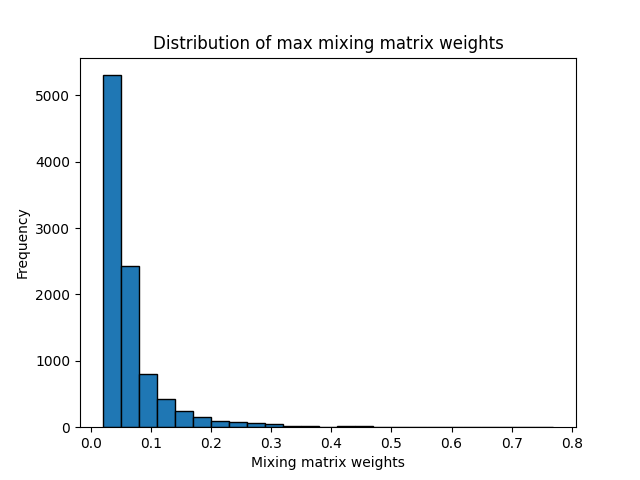
\includegraphics[scale=0.3]{mm_max}
        \caption{Distribution of maximum weights for every TC}
        \label{plt:mm_max}
    \end{subfigure}\quad
    \begin{subfigure}[t]{.3\textwidth}
        \centering
        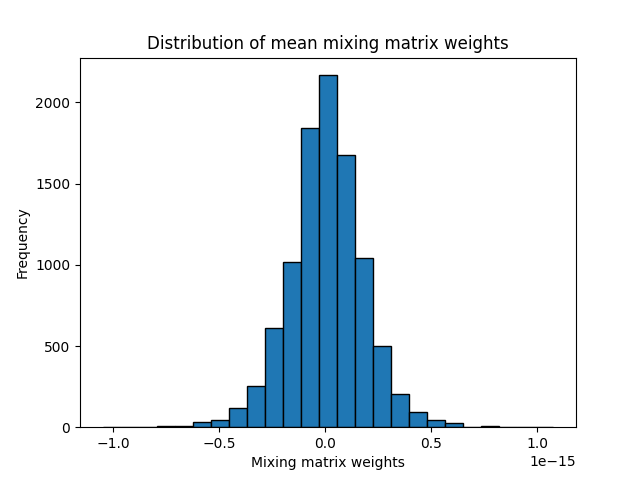
\includegraphics[scale=0.3]{mm_mean}
        \caption{Distribution of mean weights for every TC}
        \label{plt:mm_mean}
    \end{subfigure}
    \begin{subfigure}[t]{.3\textwidth}
        \centering
        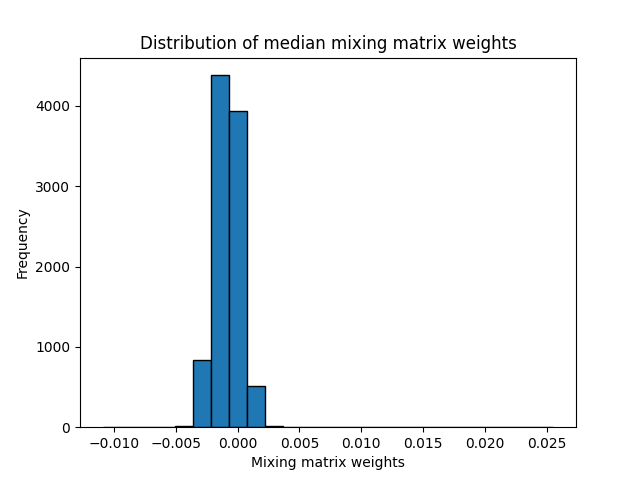
\includegraphics[scale=0.3]{mm_median}
        \caption{Distribution of median weights for every TC}
        \label{plt:mm_median}
    \end{subfigure}\quad
    \begin{subfigure}[t]{.3\textwidth}
        \centering
        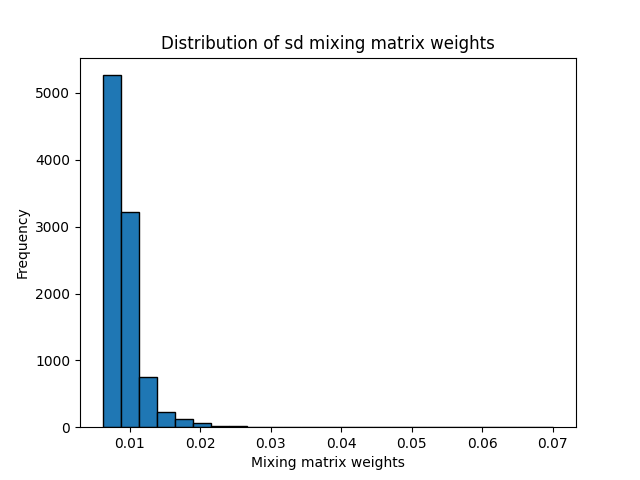
\includegraphics[scale=0.3]{mm_sd}
        \caption{Distribution of standard deviations of the weights for every TC}
        \label{plt:mm_sd}
    \end{subfigure}\quad
    \begin{subfigure}[t]{.3\textwidth}
        \centering
        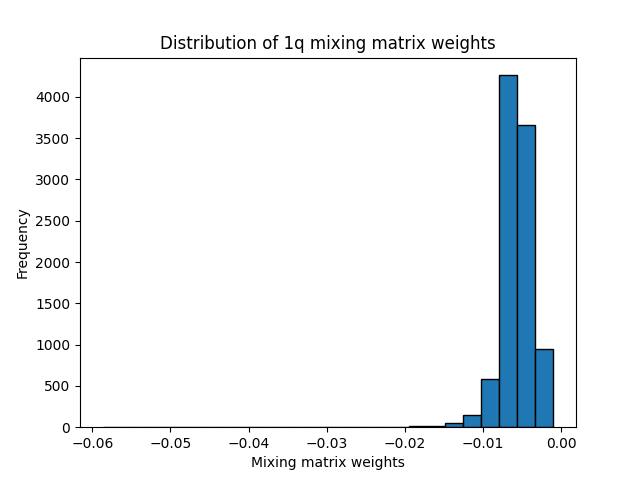
\includegraphics[scale=0.3]{mm_1q}
        \caption{Distribution of the first quartile of the weights for every TC}
        \label{plt:mm_1q}
    \end{subfigure}
    \begin{subfigure}[t]{.3\textwidth}
        \centering
        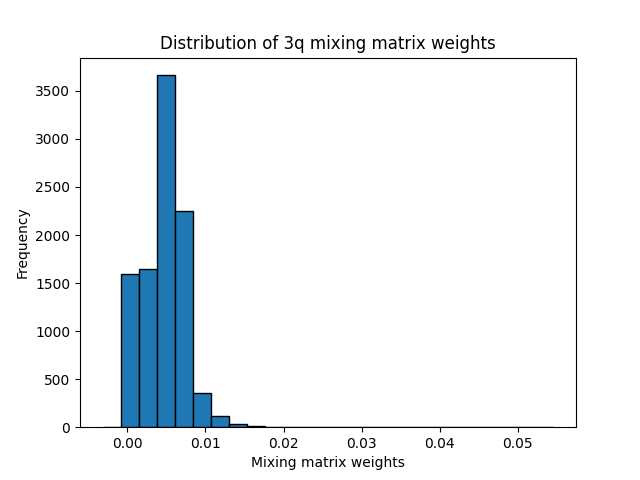
\includegraphics[scale=0.3]{mm_3q}
        \caption{Distribution of the third quartile of the weights for every TC}
        \label{plt:mm_3q}
    \end{subfigure}\quad
\caption{Histograms showcasing the distribution of mixing matrix weights for each statistic.}
\end{figure}

% TODO: better interpretation. Biological context
Figures \ref{plt:mm_min} and \ref{plt:mm_max} show a left-skewed and right-skewed distribution, respectively.
Hence, even the most extreme values in the TCs tend to be close to zero, indicating a very homogeneous dataset.
This is in line with what we expect from the normal distribution we see in figure \ref{plt:mm_mean}
The Median, 1st quartile, 3rd quartile, and standard deviation values, in figures \ref{plt:mm_median}, \ref{plt:mm_1q}, \ref{plt:mm_3q}, and \ref{plt:mm_sd} respectively, form very narrow distributions, corroborating this conclusion.

% TODO: what does 3.1g say?
Figure \ref{plt:mm_3q} has an odd shape, and I am unsure why.

Figure \ref{plt:mm_mean} looks like a normal distribution. Very nice.

\subsection{Mixing Matrix Heatmap}

% TODO: make one figure with two heatmaps: one w/ missing tumor types, one without
% still make two matplotlib figures, but remove legends with one of them
\begin{figure}[H]
    \centering
    \begin{subfigure}[t]{.3\textwidth}
        \centering
        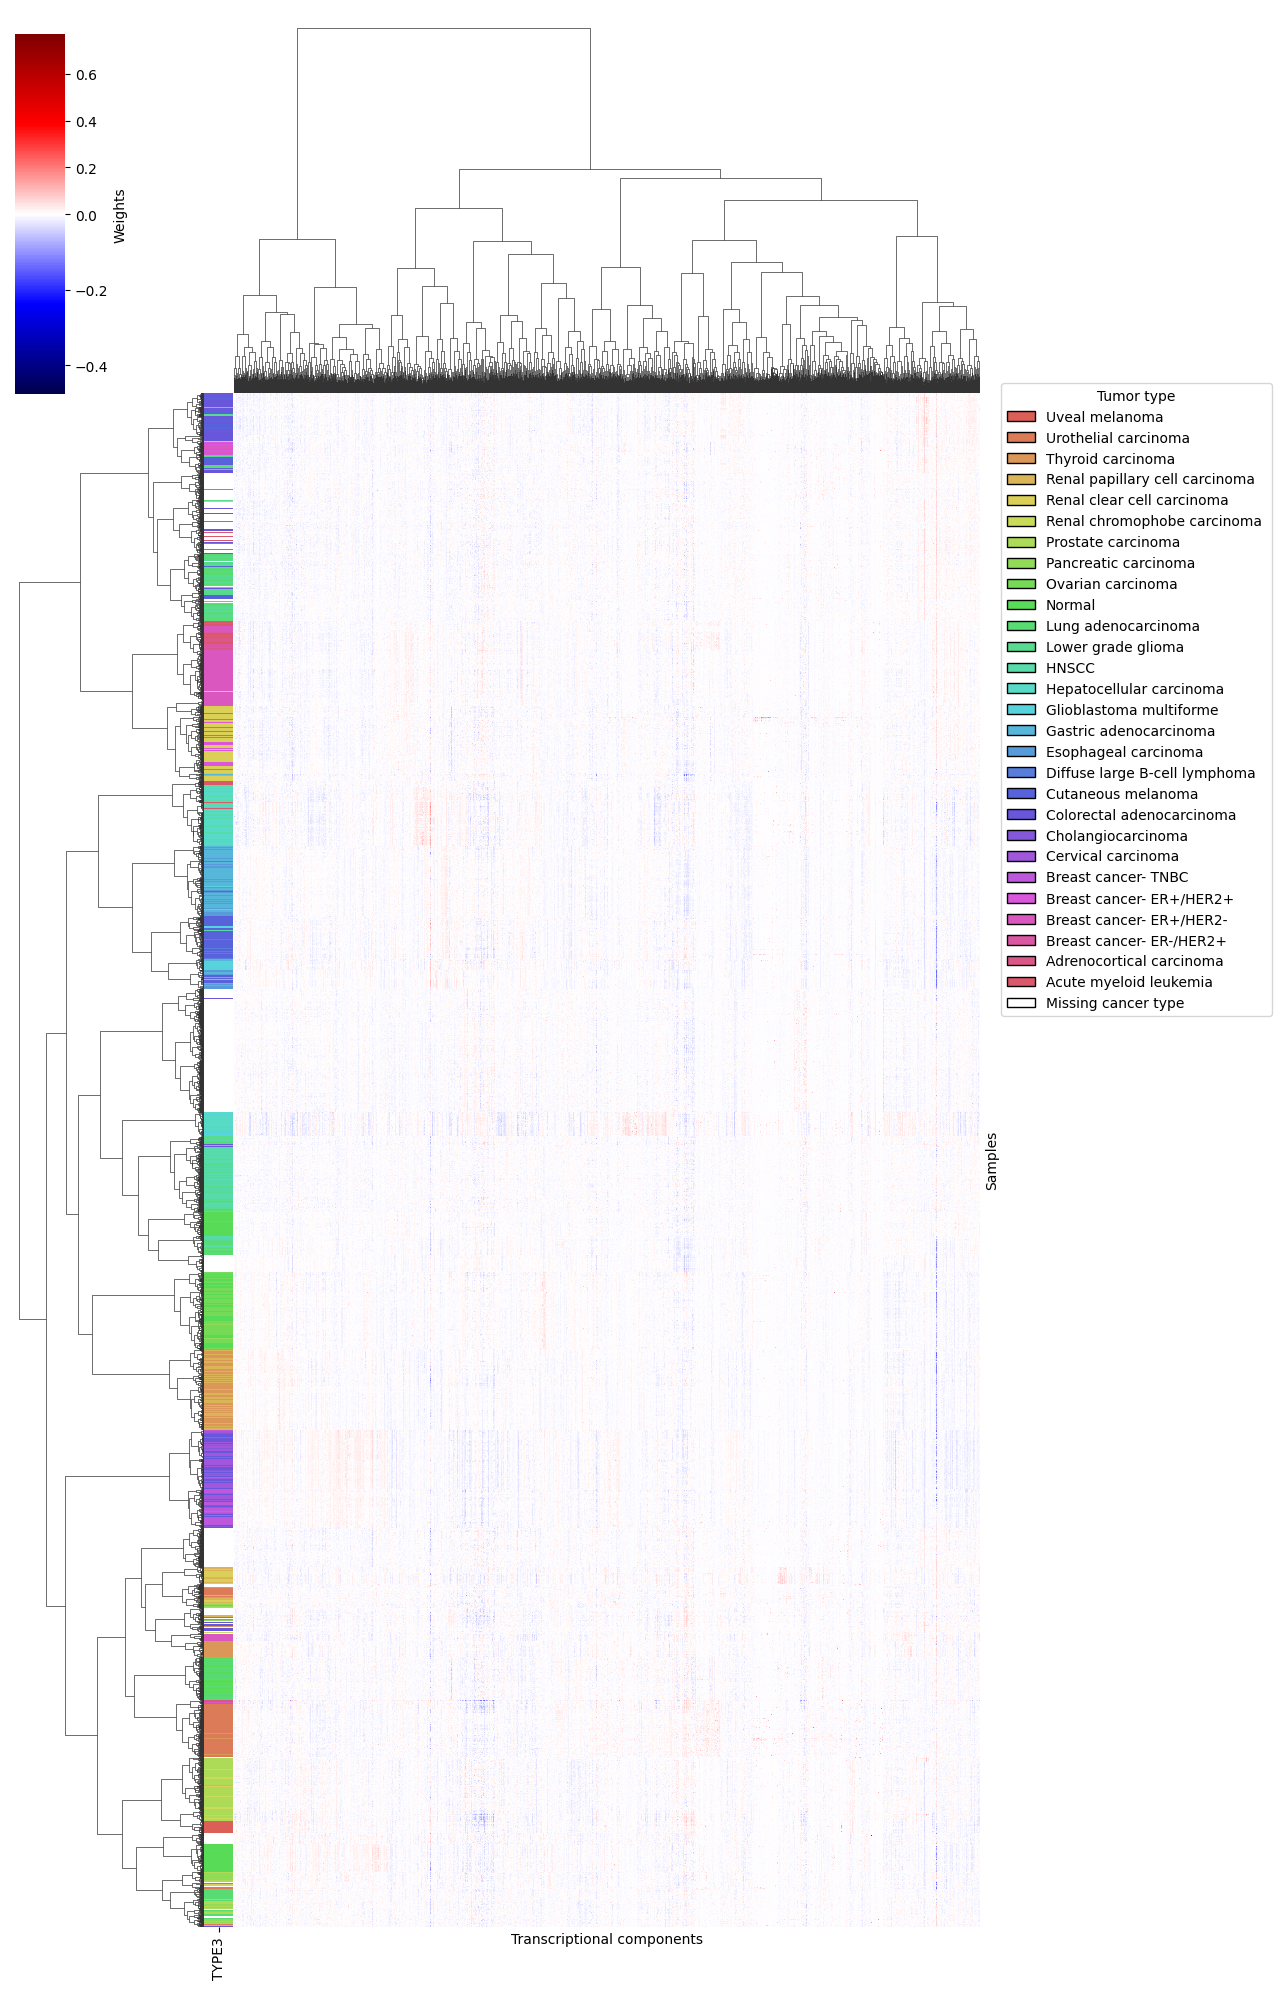
\includegraphics[scale=0.3]{images/mm_heatmap_w_missing_tt.png}
        \caption{This is a caption}
        \label{plt:mm_hm_miss_tt}
    \end{subfigure}\hspace{3cm}
    \begin{subfigure}[t]{.3\textwidth}
        \centering
        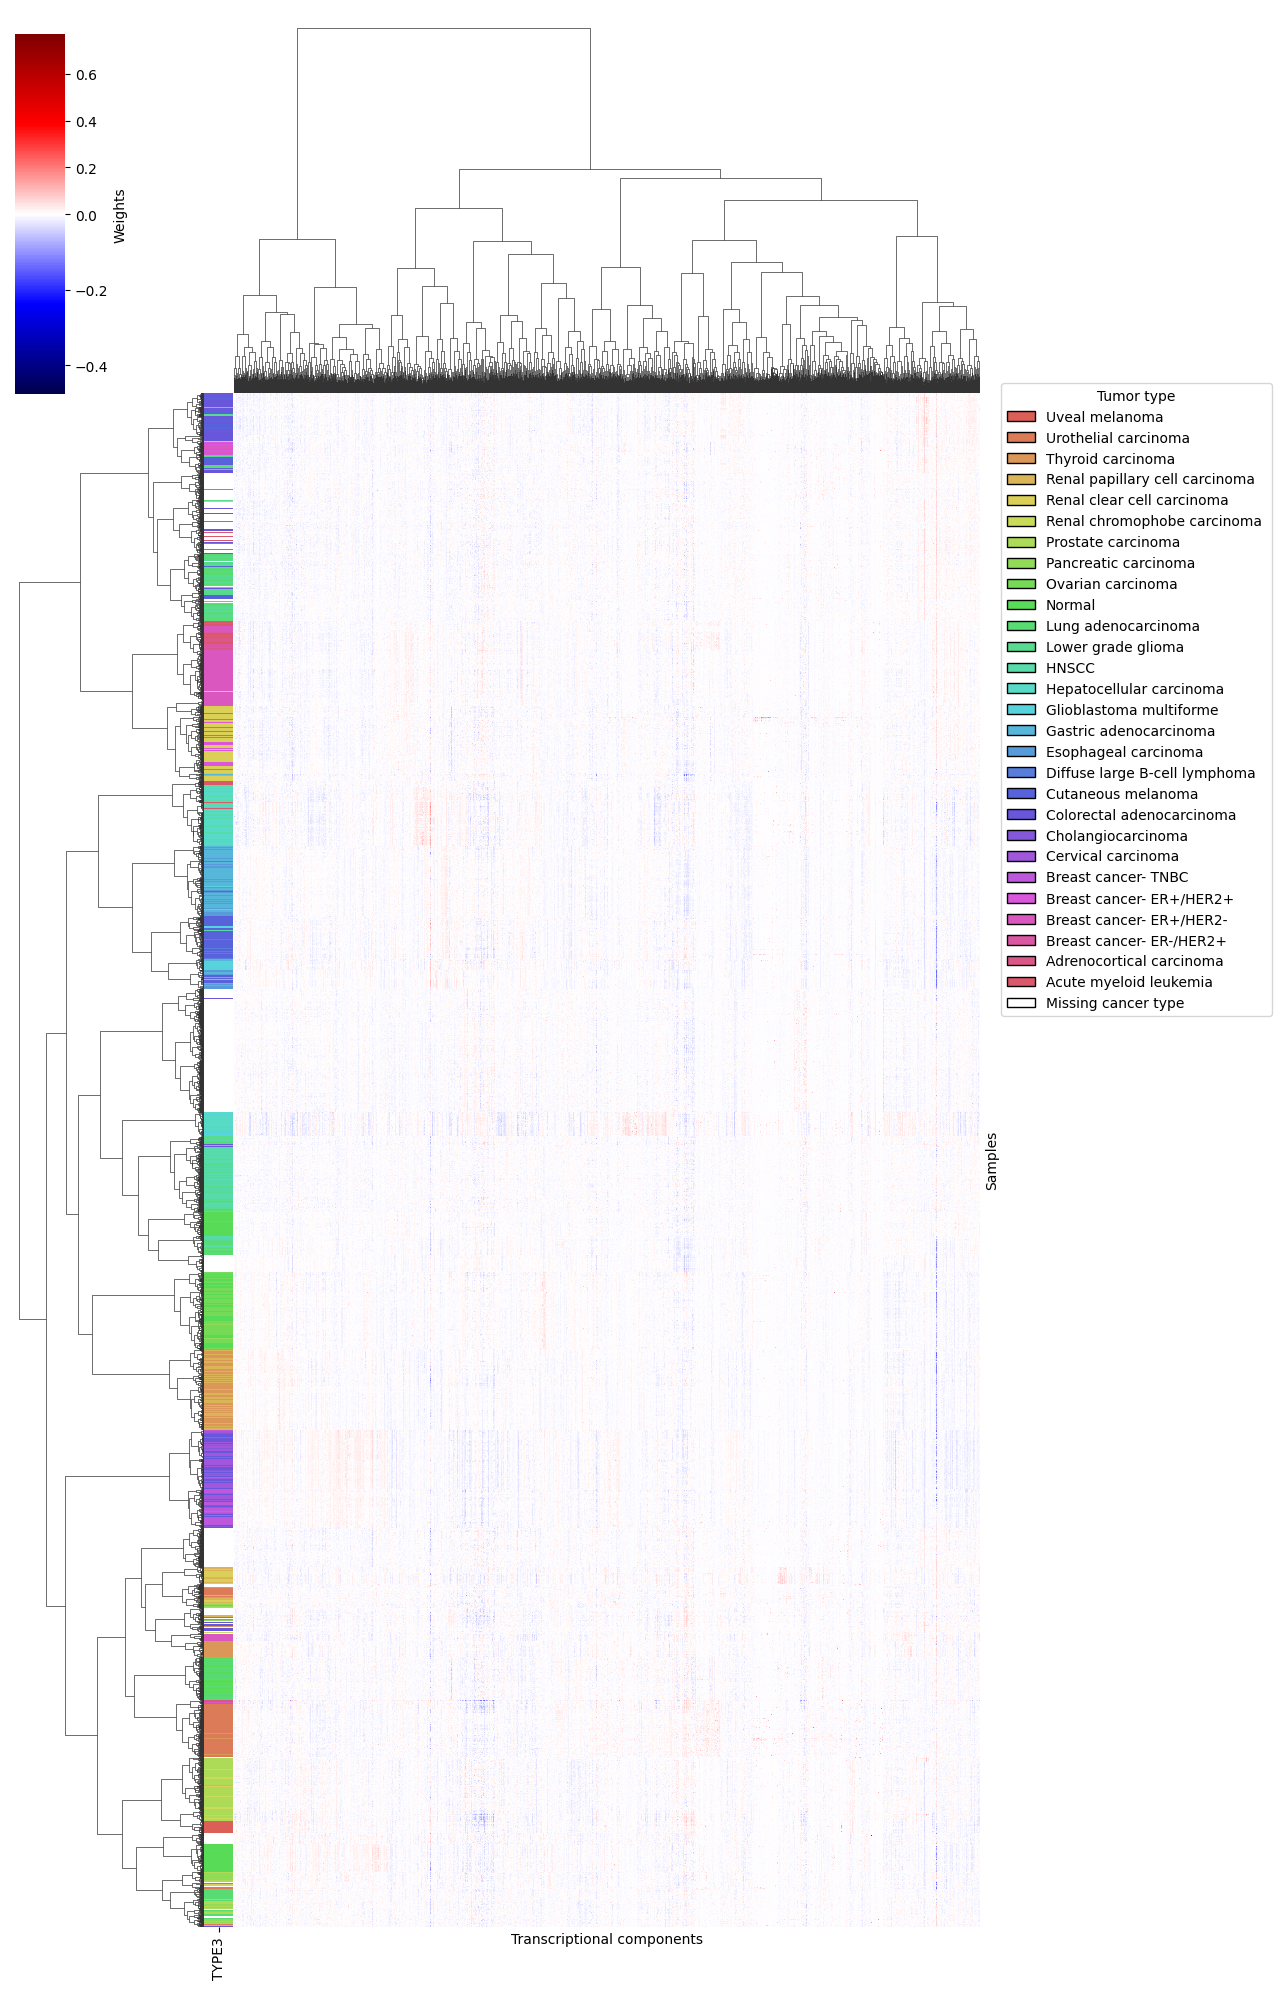
\includegraphics[scale=0.3]{images/mm_heatmap.png}
        \caption{This is also a caption}
        \label{plt:mm_hm}
    \end{subfigure}
\end{figure}

\section{Action plan}
Added a little on the outline
